\chapter{CIDR Report Analysis and Observations}

\begin{figure}
    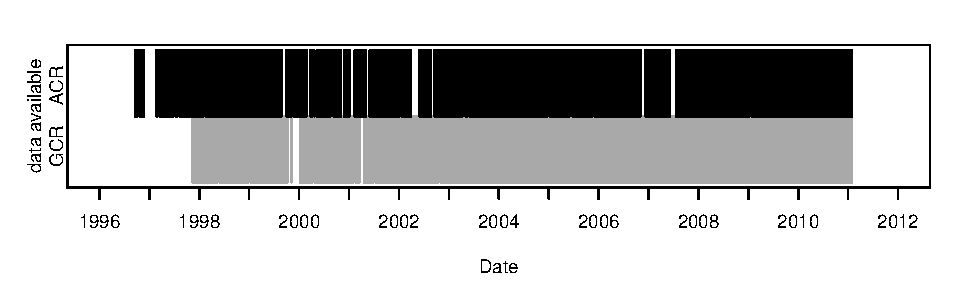
\includegraphics[width=6in]{figures/data_avail.pdf}
    \caption{Available data}
\end{figure}

\begin{figure}
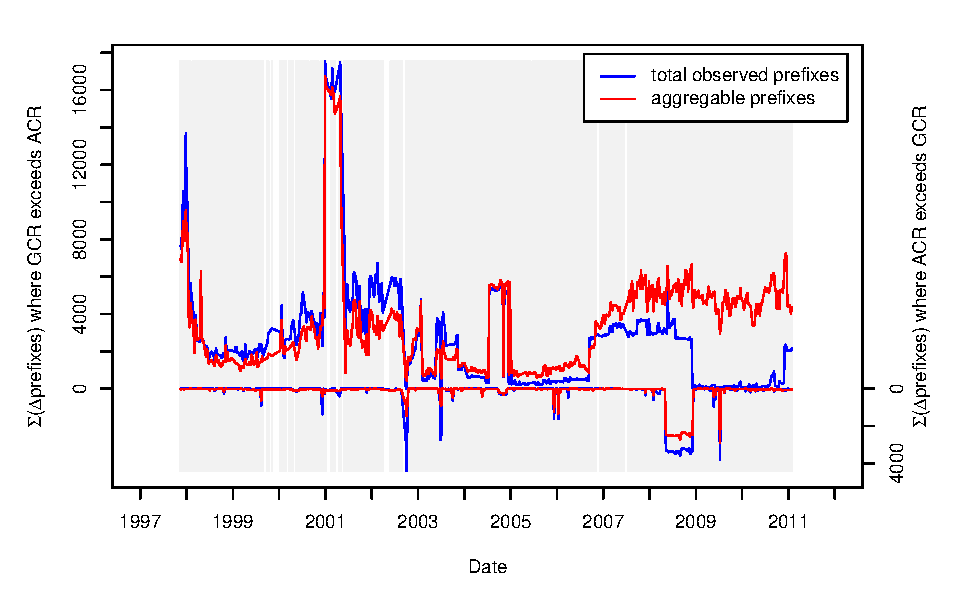
\includegraphics[width=6in]{figures/cidr_report_validity_prefix_error.pdf}
    \caption{Differences in prefix counts between authoritative (ACR) and generated (GCR) CIDR Reports over time.}
\end{figure}

\begin{figure}
    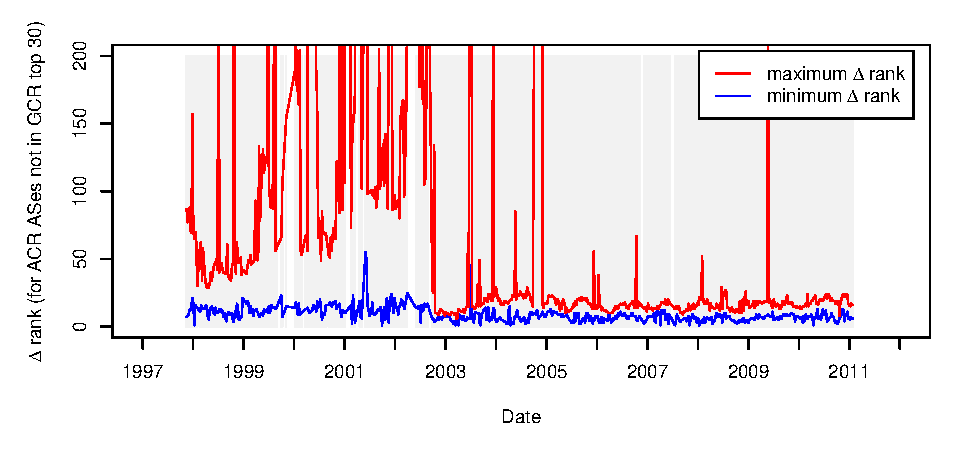
\includegraphics[width=6in]{figures/cidr_report_validity_rank_error.pdf}
    \caption{Minimum and maximum differences in ASes ranked in the top 30 on the ACR but not in the top 30 on the GCR.}
\end{figure}

\begin{figure}
    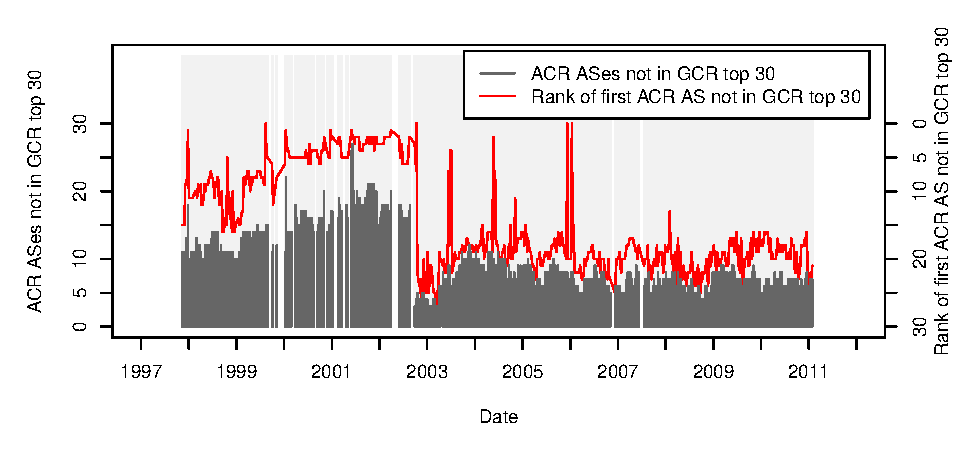
\includegraphics[width=6in]{figures/cidr_report_validity_top30_error.pdf}
    \caption{The number and first rank of ASes in the treatment group (top 30) of the ACR that are not in the treatment group of the GCR over time.}
\end{figure}

\begin{figure}
    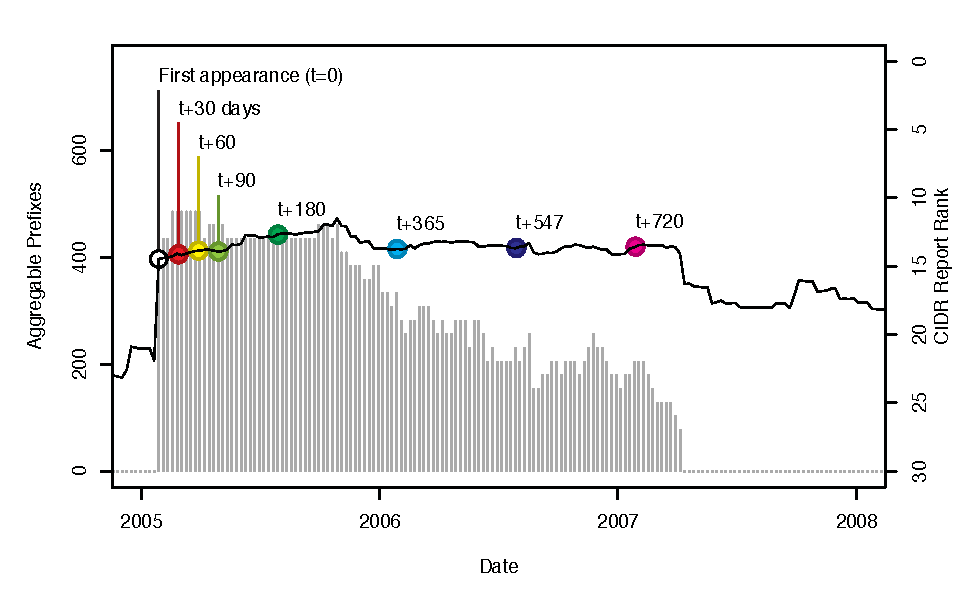
\includegraphics[width=6in]{figures/single_as.pdf}
    \caption{Measurement methodology explanation (AS 3602).}
\end{figure}

\begin{figure}
    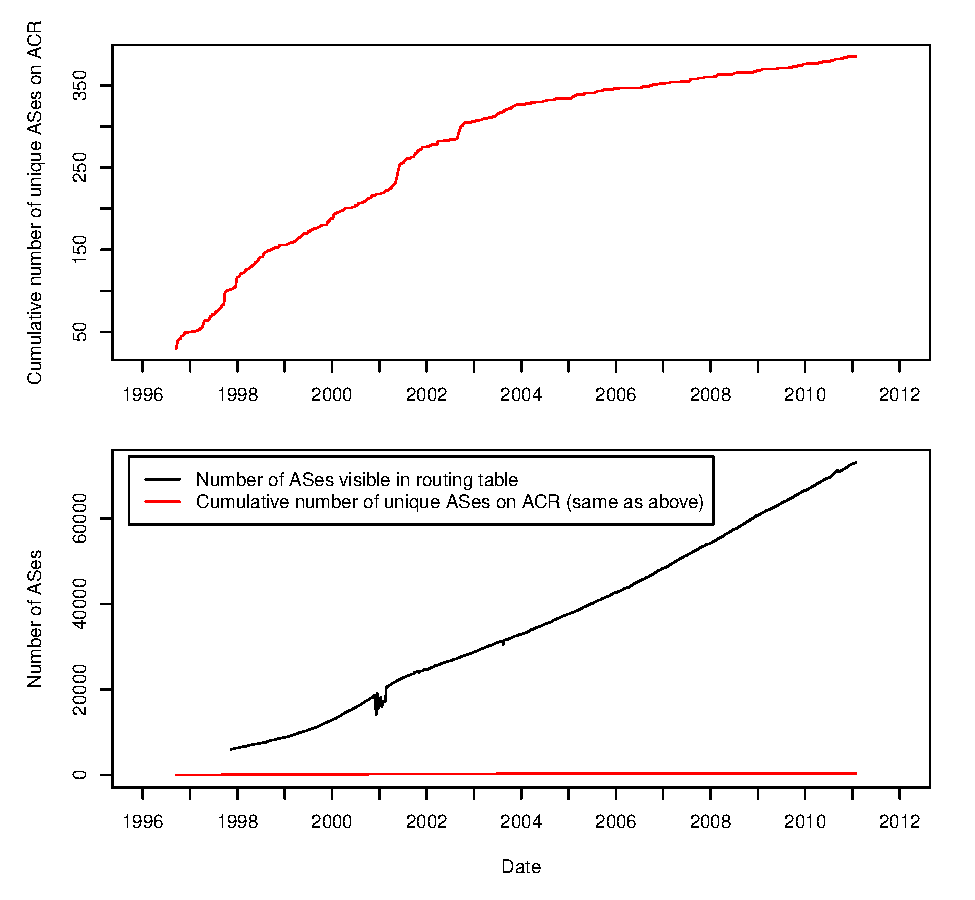
\includegraphics[width=6in]{figures/cumulative_asn_counts.pdf}
    \caption{A cumulative count of the unique ASes that have appeared on the CIDR Report and compared to the unique ASes visible in the routing table at the same moment.}
\end{figure}

\begin{figure}
    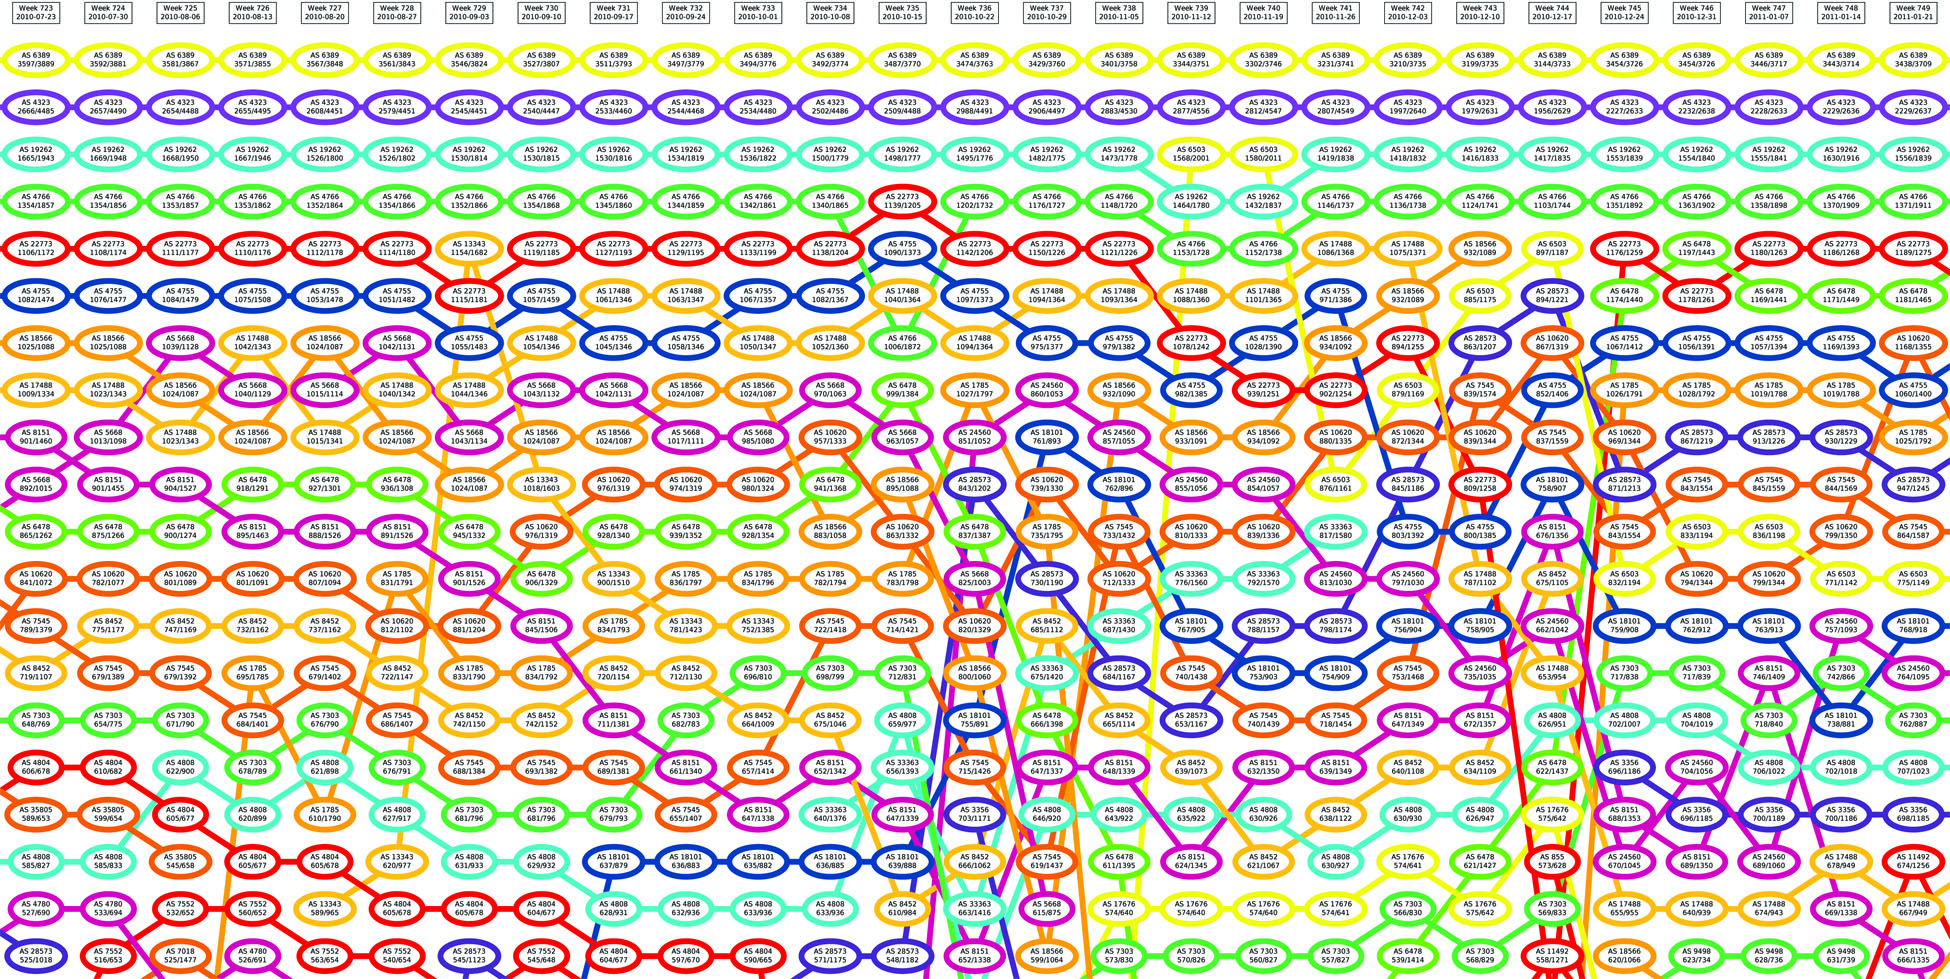
\includegraphics[width=6in]{figures/viz_sample.jpg}
    \caption{Visualization sample.}
\end{figure}




%ANALYSIS
%
%- Available data/data overview
%	- plot 'h' plots of available data
%	- plot total prefixes in the total table (Routeviews) and in the report (Cidr Report) to see that there aren't any discontinuities
%
%- Accuracy/error of my implementation of the CIDR report
%
%- Visualization of aggregate behavior and general characteristics (in particular stratification at the top of the CIDR report)
%    - Definition of metrics used in the analysis
%        - rank on CIDR Report (order by netgain)
%        - absolute/delta netgain
%        - relative/delta netgain (relative to netsnow)
%    - CDFs by AS appearnace
%    - CDFs by rank
%
%    - Summary/general statistics and characteristics of behavior over time (time series?), across and within groups, etc. (p62)
%
%- AS Behavior after appearing on the CIDR Report
%	- Distribution of AS behaviors from T=0, T=+1 month, 3 m, 6m, 1y, 2y, etc.
%		- all appearances on the cidr report
%		- no appearance/randomly selected control
%		- appearances that actually had behavior changes observed
%	- slice by date (NOT by rank on CIDR report), and by netsnow
%
%- Variance in views of data from different peers
%- for different origin ASes that appear on the CIDR Report
%- across the entire routing table
%
%////////////////////////////////////////////////////////////////////////////////
%////////////////////////////////////////////////////////////////////////////////
%////////////////////////////////////////////////////////////////////////////////
%
%DISCUSSION
%
%Discussion of the design assumptions, and the sensitivity of the CIDR report to those assumptions
